\documentclass[12pt,a4paper]{article}

% Paketler
\usepackage[utf8]{inputenc}
\usepackage[T1]{fontenc}
\usepackage[turkish,shorthands=off]{babel}
\usepackage{geometry}
\usepackage{graphicx}
\usepackage{amsmath}
\usepackage{amssymb}
\usepackage{booktabs}
\usepackage{hyperref}
\usepackage{cite}
\usepackage{setspace}
\usepackage{url}
\usepackage{subcaption}
\usepackage{float}

% Sayfa ayarları
\geometry{margin=2.5cm}
\onehalfspacing

\hypersetup{
    colorlinks=true,
    linkcolor=blue,
    filecolor=magenta,      
    urlcolor=cyan,
    pdftitle={Dermoskopik Goruntulerde Melanom Tespiti icin Ikili Siniflandirma},
    pdfpagemode=FullScreen,
}

% Başlık bilgileri
\title{
    \large\textbf{İZMİR BAKIRÇAY ÜNİVERSİTESİ}\\
    \large Mühendislik ve Mimarlık Fakültesi\\
    \large Bilgisayar Mühendisliği Bölümü\\
    \vspace{0.5cm}
    \large\textit{Yapay Zeka ve Derin Öğrenme Dersi}\\
    \vspace{1.5cm}
    \huge\textbf{Dermoskopik Görüntülerde Melanom Tespiti için İkili Sınıflandırma}\\
    \vspace{0.5cm}
    \large\textbf{ISIC 2020 Veri Seti Üzerinde Transfer Öğrenme Yaklaşımı}
}

\author{
    \textbf{Utku Aydın}\\
    Öğrenci No: 6053037\\
    6053041@bakircay.edu.tr\\
    \\
    \textbf{Utku Dişci}\\
    Öğrenci No: 6053041\\
    6053041@bakircay.edu.tr\\
    \\
    \textbf{Danışman:}\\
    Dr. Öğr. Üyesi Nihan Özbaltan\\
    Bilgisayar Mühendisliği Bölümü
}

\date{Mayıs 2026}

\begin{document}

\maketitle
\newpage

\begin{abstract}
\noindent Deri kanseri, özellikle metastaz potansiyeli nedeniyle melanomun agresif doğası gereği önemli bir küresel sağlık sorunudur. Erken teşhis, hayatta kalma oranlarını dramatik şekilde artırır; ileri evrelerde \%20'lere düşen oran, erken evrede yaklaşık \%99'a ulaşır. Bu nedenle, doğru ve zamanlı sınıflandırma sistemleri klinik pratik için hayati öneme sahiptir.

Bu çalışma, dermoskopik görüntülerden otomatik ikili sınıflandırma yaparak melanom tespiti için derin öğrenme çerçevesi sunmaktadır. İki tanısal kategoriyi (iyi huylu lezyonlar ve melanom) içeren ISIC 2020 Yarışma Veri Seti'ndeki 33.126 dermoskopik görüntüyü kullandık. Veri seti, iyi huylu lezyonların yaklaşık \%98,2'sini oluşturduğu ve melanomun sadece \%1,8'ini temsil ettiği ciddi bir sınıf dengesizliği sergilemektedir.

Bu zorlukları ele almak için, ImageNet üzerinde önceden eğitilmiş ResNet-50 ve EfficientNet-V2-S mimarilerini focal loss optimizasyonu, ağırlıklı rastgele örnekleme ve stratejik veri bölme ile birleştirdik. Yaklaşımımız, klinik açıdan en güvenli kabul edilen \%50 eşik değerinde \%87,81 genel doğruluk ve melanom tespiti için 0,8940 AUC-ROC değeri elde ederek son derece başarılı sonuçlar göstermiştir.

Geliştirilen sistem, klinik karar destek aracı olarak tasarlanmış olup, özellikle kaynakları sınırlı ortamlarda dermatologlara destek sağlamak ve tanısal değişkenliği azaltmak amacıyla objektif bir ikinci görüş sunmaktadır.
\vspace{0.5cm}

\noindent\textbf{Anahtar Kelimeler:} Melanom tespiti, cilt lezyonu sınıflandırması, dermoskopi, evrişimli sinir ağları, transfer öğrenme, ISIC 2020, focal loss, sınıf dengesizliği, ağırlıklı örnekleme, derin öğrenme.
\end{abstract}

\newpage

\section{Giriş}
\label{sec:giris}

\subsection{Arka Plan ve Motivasyon}
\label{subsec:arka_plan}

Cilt kanseri, dünya genelinde insidansı hızla artan malignitelerin başında gelmektedir. Özellikle habis melanom, diğer deri kanseri türlerine göre çok daha az görülmesine karşın, lenf ve kan yoluyla uzak organlara metastaz yapma eğilimi nedeniyle ölümlerin büyük bir kısmından sorumludur. Erken evrelerde tespit edilen melanom vakalarında beş yıllık sağkalım oranı yaklaşık \%99 iken, geç evre veya metastaz yapmış hastalarda bu oran \%20'lere kadar gerilemektedir~\cite{esteva2017}. Dolayısıyla, erken teşhis melanom yönetiminde en kritik hayatta kalma faktörüdür.

Klinik pratikte dermatologlar, asimetri, sınır düzensizliği, renk çeşitliliği, çap ve gelişim (ABCD) kriterlerini kullanarak dermoskopik görüntüler üzerinden görsel muayene yapmaktadır. Ancak bu teşhis yöntemi son derece subjektiftir; dermatoloğun deneyimine, dikkat durumuna ve cihaz kalitesine doğrudan bağlıdır. Deneyimli klinisyenler arasında bile tanısal kararlarda yüksek oranda değişkenlik gözlenebilmektedir. Bu sınırlamalar, dermatologlara karar verme sürecinde yardımcı olabilecek, nesnel, ölçeklenebilir ve yüksek doğruluklu otomatik bilgisayar destekli tanı (CAD) sistemlerine olan ihtiyacı ortaya çıkarmıştır.

\subsection{Literatür Taraması}
\label{subsec:literatur}

Son yıllarda derin öğrenme, bilgisayarlı görü ve tıbbi görüntüleme alanlarında devrim niteliğinde başarılar sağlamıştır. \textit{Nature} dergisinde yayınlanan öncü çalışmasında Esteva ve ark.~\cite{esteva2017}, 129.450 dermoskopik görüntüden oluşan devasa bir veri seti üzerinde uçtan uca eğittikleri tek bir Evrişimli Sinir Ağı (CNN) modelinin, 21 diplomalı uzman dermatolog ile başa baş ikili sınıflandırma performansı sergilediğini kanıtlamıştır.

Bu başarıyı takiben, Haenssle ve ark.~\cite{haenssle2018} tarafından yürütülen prospektif bir okuyucu çalışmasında, geliştirilen CNN tabanlı yapay zeka sisteminin, testi gerçekleştiren 58 dermatoloğun büyük bir kısmından (özellikle daha az deneyimli olanlardan \%71,3 ve deneyimli olanlardan \%75,7 hassasiyet oranlarına kıyasla \%82,5 duyarlılık ile) daha yüksek bir başarı gösterdiği bildirilmiştir. Brinker ve ark.~\cite{brinker2019} ise yaptıkları sistematik derlemede, derin öğrenme sistemlerinin cilt lezyonlarının ikili sınıflandırılmasında tutarlı bir şekilde dermatologlara karşı üstün ya da en azından eşdeğer performans gösterdiğini ortaya koymuştur.

Son dönemdeki çalışmalar ise model mimarilerinin parametre verimliliğini artırmaya odaklanmıştır. Tan ve Le~\cite{tan2019} tarafından geliştirilen EfficientNet ailesi, ağın derinliğini, genişliğini ve girdi çözünürlüğünü dengeli bir şekilde ölçeklendiren ``Bileşik Ölçeklendirme'' (Compound Scaling) yöntemini literatüre kazandırmıştır. Bu mimarinin bir sonraki sürümü olan EfficientNet-V2~\cite{tan2021}, aşamalı öğrenme (progressive learning) ve hızlı sinir mimarisi araması (NAS) ile çok daha küçük parametre boyutlarında ve çok daha hızlı eğitim sürelerinde üstün başarı elde etmeyi başarmıştır. Bunun yanı sıra Lin ve ark.~\cite{lin2017} tarafından önerilen Focal Loss fonksiyonu, tıbbi görüntülemedeki en büyük engellerden biri olan aşırı sınıf dengesizliğini çözmek amacıyla kolay sınıflandırılan örneklerin kaybını baskılayarak zor örneklere odaklanmaktadır.

\subsection{Araştırma Problemi}
\label{subsec:problem}

Tıbbi yapay zeka sistemlerinin klinik ortama başarıyla aktarılabilmesinin önünde birtakım teknik ve operasyonel engeller bulunmaktadır:
\begin{enumerate}
    \item \textbf{Aşırı Sınıf Dengesizliği:} ISIC 2020 veri seti gibi halka açık büyük veri setlerinde, iyi huylu (benign) vakaların oranı \%98'in üzerinde iken kanserli (malignant) vaka oranı \%2'nin altındadır. Bu durum, standart çapraz entropi kaybı kullanan modellerin ezbere ``iyi huylu'' sınıfını tahmin etmesine ve kanser vakalarını kaçırmasına (yüksek False Negative) yol açar.
    \item \textbf{Donanımsal Sınırlılıklar ve Mobil Dağıtım:} Birçok büyük model (ResNet-50, ViT vb.) on milyonlarca parametre barındırmakta ve yüksek bellek/işlemci gücüne ihtiyaç duymaktadır. Klinik ortamlardaki veya taşınabilir cihazlardaki kısıtlı kaynaklar altında çalışabilecek verimli, hafif ve buna rağmen yüksek performanslı modellere ihtiyaç vardır.
\end{enumerate}

\subsection{Önerilen Yaklaşım}
\label{subsec:yaklasim}

Bu çalışmada, yukarıda bahsedilen zorlukları aşmak adına, transfer öğrenme (Transfer Learning) tabanlı, sınıf dengesizliğine duyarlı ve donanım dostu bir melanom tespit çerçevesi önerilmektedir. Önerilen sistem:
\begin{itemize}
    \item ImageNet üzerinde önceden eğitilmiş \textbf{EfficientNet-V2-S} mimarisini temel alır.
    \item Mini-grup bazında örnek dengesini sağlamak için \textbf{Ağırlıklı Rastgele Örnekleme} (Weighted Random Sampling) yöntemini entegre eder.
    \item Kanser gibi azınlık sınıfların doğru sınıflandırılmasını teşvik etmek üzere optimize edilmiş \textbf{Focal Loss} ($\alpha=0,85, \gamma=2,0$) kayıp fonksiyonunu kullanır.
    \item Modelin güvenilirliğini ve genelleme yeteneğini artırmak için geniş kapsamlı \textbf{fotometrik veri artırma} stratejileri uygular.
\end{itemize}

\subsection{Katkılar}
\label{subsec:katkilar}

Bu makalenin temel özgün katkıları aşağıdaki gibidir:
\begin{enumerate}
    \item Aşırı derecede sınıf dengesizliğine (98:2 oranı) sahip ISIC 2020 veri seti üzerinde, parametre dostu \textbf{EfficientNet-V2-S} ve geleneksel \textbf{ResNet-50} modellerinin başarımı karşılaştırmalı olarak analiz edilmiştir.
    \item \textbf{Focal Loss} ve \textbf{Ağırlıklı Rastgele Örnekleme} kombinasyonunun, kanserli vakaları yakalamadaki (Recall/Duyarlılık) kritik rolü deneysel olarak kanıtlanmıştır.
    \item Algoritmik veri sızıntılarını önlemek amacıyla SHA-256 tabanlı yinelenen görsel eleme boru hattı tasarlanmıştır.
    \item Klinik tarama (screening) senaryoları göz önüne alınarak, farklı karar sınırlarında (\%50, \%75, \%85) ayrıntılı klinik duyarlılık analizleri gerçekleştirilmiştir.
    \item Apple Metal Performance Shaders (MPS) ve NVIDIA CUDA donanım hızlandırıcıları üzerinde çalışabilen çapraz platform uyumlu bir altyapı oluşturulmuştur.
\end{enumerate}

\subsection{Makale Yapısı}
\label{subsec:makale_yapisi}

Makalenin geri kalan kısımları şu şekilde organize edilmiştir: Bölüm~\ref{sec:ilgili_calismalar}'de dermatolojide derin öğrenme uygulamaları ve ilgili literatür özetlenmektedir. Bölüm~\ref{sec:materyal_yontem}'de veri seti, boru hattı, model mimarileri ve eğitim detayları sunulmaktadır. Bölüm~\ref{sec:bulgular}'da deneysel bulgular, elde edilen sayısal sonuçlar ve performans grafikleri analiz edilmektedir. Bölüm~\ref{sec:tartisma}'da klinik çıkarımlar, kısıtlar ve gelecek hedefler tartışılmakta ve Bölüm~\ref{sec:sonuc}'ta çalışma sonlandırılmaktadır.

\section{İlgili Çalışmalar}
\label{sec:ilgili_calismalar}

\subsection{Dermatolojide Derin Öğrenme}
Dermatolojik lezyonların görsel yapısı (renk, doku, kenar düzensizliği), CNN'lerin öznitelik çıkarma yeteneğine son derece uygundur. Esteva ve ark.~\cite{esteva2017}'nın ardından, birçok araştırmacı farklı lezyon tiplerini (bazal hücreli karsinom, aktinik keratoz vb.) ayırt edebilen çok sınıflı modeller geliştirmiştir. Ancak bu modellerin gerçek hastane ortamlarında genellenebilirlik sorunu yaşadığı ve klinisyenlerin yerini almaktan ziyade karar destek sistemi olarak konumlandırılması gerektiği anlaşılmıştır.

\subsection{Tıbbi Görüntüleme için Transfer Öğrenme}
Tıbbi görüntüleme alanındaki en büyük sınırlılık, etiketli kaliteli veri miktarının azlığıdır. Bu sorunu çözmek için doğal görüntülerden (ImageNet) öğrenilen ağırlıkların tıbbi görüntülere aktarılması (Transfer Learning) standart bir uygulama haline gelmiştir. Bu sayede model, sıfırdan eğitilmek yerine temel kenar, doku ve kontrast bilgilerini hazır olarak almakta ve tıbbi göreve çok daha hızlı uyum sağlamaktadır.

\subsection{Tıbbi Sınıflandırmada Sınıf Dengesizliği}
Nadir görülen hastalıkların tespiti doğası gereği dengesiz veri kümesi yaratır. Literatürde bu soruna yönelik veri düzeyinde (aşırı örnekleme - SMOTE) ve algoritma düzeyinde (maliyete duyarlı kayıp fonksiyonları) çözümler önerilmiştir. Lin ve ark.~\cite{lin2017}'nın önerdiği Focal Loss, özellikle nesne tespiti dışında tıbbi görüntü sınıflandırma görevlerinde de kolay arka plan (sağlıklı doku) örneklerini baskılayarak kanserli bölgelere odaklanmada üstün başarısını kanıtlamıştır.

\subsection{Veri Bütünlüğü ve Tekrar Edilebilirlik}
Tıbbi veri setlerinde mükerrer görsel bulunması (aynı hastadan farklı açılardan alınmış görüntüler gibi) veri sızıntılarına (data leakage) ve yapay yüksek başarılara neden olur. Son literatür, veri bütünlüğünün sağlanması için SHA-256 gibi algoritmalarla veri tekilleştirme yapılmasının önemine odaklanmaktadır~\cite{rotemberg2021}.

\section{Materyal ve Yöntem}
\label{sec:materyal_yontem}

\subsection{Veri Seti}
Bu çalışmada kullanılan veri seti, Uluslararası Cilt Görüntüleme İşbirliği (ISIC) tarafından sağlanan halka açık \textbf{ISIC 2020 Challenge} veri kümesidir~\cite{rotemberg2021}. Toplamda \textbf{33.126 dermoskopik görüntü} içeren veri kümesinde sınıfların dağılımı şu şekildedir:
\begin{itemize}
    \item \textbf{İyi Huylu (Benign):} 32.528 görsel ($\sim$\%98,2)
    \item \textbf{Habis Melanom (Malignant):} 598 görsel ($\sim$\%1,8)
\end{itemize}
Görüntüler, Kaggle platformunda optimize edilmiş 256$\times$256 piksel çözünürlüğündeki JPEG formatında temin edilmiştir~\cite{kaggle2020}.

\subsection{Veri Bütünlüğü Boru Hattı}

\subsubsection{Tekrar Tespiti (Duplicate Detection)}
Aynı lezyonun farklı açılardan çekilmiş mükerrer nüshalarını veya eğitim kümesi ile doğrulama kümesi arasına sızabilecek aynı görselleri temizlemek amacıyla bir SHA-256 hash boru hattı kurulmuştur. Eşleşen hash değerine sahip birebir kopyalar veri kümesinden elenerek modelin ezberleme oranları kontrol altında tutulmuştur.

\subsubsection{Stratejik Bölme (Stratified Splitting)}
Sınıf oranlarının korunması ve doğrulama kümesinde yeterli miktarda melanom örneğinin bulunması için \textbf{Tabakalı Bölme} (Stratified Split) uygulanmıştır. Veri seti rastgele bir tohum değeri belirlenerek (seed=42) \%80 eğitim ve \%20 doğrulama (validation) olarak ikiye ayrılmıştır.

\subsection{Ön İşleme ve Artırma}

\subsubsection{Normalizasyon}
Tüm görseller öncelikle model girdisi olarak 224$\times$224 piksel çözünürlüğüne dönüştürülmüştür. Ardından ImageNet veri kümesinin kanal bazlı istatistikleri kullanılarak normalize edilmiştir:
\begin{equation}
    I_{norm} = \frac{I - \mu}{\sigma}
\end{equation}
Burada $\mu = [0,485; 0,456; 0,406]$ ve $\sigma = [0,229; 0,224; 0,225]$ olarak tanımlanmıştır.

\subsubsection{Veri Artırma}
Modelin dönme, ışık ve açı farklarına karşı dayanıklı olabilmesi amacıyla eğitim kümesinde şu fotometrik artırımlar uygulanmıştır:
\begin{itemize}
    \item Rastgele Yatay ve Dikey Çevirme ($p=0,5$)
    \item Rastgele Döndürme ($-20^\circ$ ile $+20^\circ$ arası)
    \item Renk Değişimleri (Brightness, Contrast, Hue, Saturation faktörleri $[0,8; 1,2]$ aralığında)
\end{itemize}

\subsection{Model Mimarileri}

\subsubsection{ResNet-50}
Derin CNN'lerde yaşanan kaybolan gradyan (vanishing gradient) problemini aşmak amacıyla He ve ark.~\cite{he2016} tarafından geliştirilen ResNet-50, atlama bağlantıları (residual connections) içeren 50 katmanlı güçlü bir modeldir. 25,6 milyon parametreye sahiptir ve transfer öğrenme kıyaslamalarında güçlü bir baseline oluşturmaktadır.

\subsubsection{EfficientNet-V2-S}
Google tarafından sunulan EfficientNet-V2-S, akıllı ölçeklendirme mantığı ile hem yüksek doğruluk hem de yüksek eğitim verimliliği sağlamaktadır. Fused-MBConv blokları içeren model, 21,5 milyon parametresiyle ResNet-50'den \%20 daha küçüktür. Son sınıflandırma katmanı, melanom ikili tespiti için tek bir nöron ve sigmoid aktivasyonuna sahip olacak şekilde değiştirilmiştir.

\subsection{Eğitim Stratejisi}

\subsubsection{Sınıf Dengesizliğini Azaltma}
Aşırı dengesiz veri kümesini yönetmek için iki önemli strateji bir arada kullanılmıştır:
\begin{enumerate}
    \item \textbf{Ağırlıklı Rastgele Örnekleme (Weighted Random Sampler):} Eğitim gruplarında (batches) her iki sınıftan dengeli sayıda görsel bulunması amacıyla her $c$ sınıfındaki örneğe şu ağırlık ($w_c$) atanmıştır:
    \begin{equation}
        w_c = \frac{N}{N_c \times C}
    \end{equation}
    Burada $N$ toplam eğitim örneği, $N_c$ ilgili sınıftaki örnek sayısı ve $C$ toplam sınıf sayısıdır ($C=2$).
    \item \textbf{Focal Loss:} Standart ikili çapraz entropi kaybı yerine kullanılan Focal Loss şu şekilde formüle edilmiştir:
    \begin{equation}
        FL(p_t) = -\alpha_t (1 - p_t)^\gamma \log(p_t)
    \end{equation}
    Burada $\alpha_t=0,85$ (kanser sınıfına verilen yüksek ağırlık) ve $\gamma=2,0$ (kolay örneklerin etkisini azaltan odaklama parametresi) olarak seçilmiştir.
\end{enumerate}

\subsubsection{Optimizasyon Yapılandırması}
Modeller AdamW optimizasyon algoritması kullanılarak $10^{-4}$ sabit öğrenme oranı (learning rate) ve 32 batch size ile 30 epoch boyunca eğitilmiştir. Doğrulama AUC değerine dayalı erken durdurma (early stopping) uygulanmış ve en iyi ağırlıklar (\texttt{best\_model.pth}) kaydedilmiştir.

\subsubsection{Çapraz Platform Uyumluluğu}
Yazılan derin öğrenme kodu donanımı otomatik olarak algılar:
\begin{equation}
    \text{Device} = \begin{cases} 
      \text{cuda} & \text{NVIDIA GPU mevcutsa} \\
      \text{mps} & \text{Apple Silicon GPU mevcutsa} \\
      \text{cpu} & \text{Diğer durumlarda}
   \end{cases}
\end{equation}
Bu sayede Windows iş istasyonlarında CUDA, macOS sistemlerde ise Apple Metal API'si yardımıyla MPS tabanlı tam GPU hızlandırma sağlanmıştır.

\subsection{Değerlendirme Metrikleri}
Model performansını ölçmek için doğruluk (Accuracy), kesinlik (Precision), duyarlılık (Recall/Sensitivity), F1-Skoru ve ROC-AUC (Eğri Altındaki Alan) kullanılmıştır:
\begin{equation}
    \text{Doğruluk} = \frac{TP + TN}{TP + TN + FP + FN}
\end{equation}
\begin{equation}
    \text{Duyarlılık (Recall)} = \frac{TP}{TP + FN}
\end{equation}
\begin{equation}
    \text{Kesinlik (Precision)} = \frac{TP}{TP + FP}
\end{equation}
\begin{equation}
    \text{F1-Skoru} = 2 \times \frac{\text{Precision} \times \text{Recall}}{\text{Precision} + \text{Recall}}
\end{equation}

\subsubsection{Çoklu Eşik Analizi}
Farklı klinik önceliklere (örneğin kanserli hastayı kaçırmamak adına yanlış alarmları kabul etmek veya tam tersi) uyum sağlamak üzere modeller \%50, \%75 ve \%85 olasılık eşiklerinde değerlendirilmiştir.

\section{Bulgular}
\label{sec:bulgular}

\subsection{Deneysel Kurulum}
Deneyler PyTorch 2.1 framework'ü kullanılarak Windows üzerinde NVIDIA RTX serisi discrete GPU'larda ve Apple Silicon donanımında gerçekleştirilmiştir. Eğitim süresi toplamda her iki model için yaklaşık 16 saattir.

\subsection{Model Performansı}
ResNet-50 ve EfficientNet-V2-S modellerinin ISIC 2020 doğrulama veri kümesi üzerindeki genel performans sonuçları Tablo~\ref{tab:model_performans}'de karşılaştırmalı olarak sunulmuştur.

\begin{table}[H]
\centering
\caption{ISIC 2020 Doğrulama Kümesi Üzerinde İkili Sınıflandırma Performansı}
\label{tab:model_performans}
\resizebox{\textwidth}{!}{%
\begin{tabular}{lccccc}
\toprule
\textbf{Model Mimarisi} & \textbf{Doğruluk} & \textbf{Kesinlik} & \textbf{Duyarlılık} & \textbf{F1-Skoru} & \textbf{AUC-ROC} \\
\midrule
ResNet-50 (Epoch 5) & \%87,90 & \%9,83 & \%72,65 & \%17,32 & \%90,00 \\
EfficientNet-V2-S (Epoch 1) & \%87,81 & \%9,93 & \%74,36 & \%17,52 & \%89,40 \\
\bottomrule
\end{tabular}%
}
\end{table}

Tablo~\ref{tab:model_performans} incelendiğinde, iki modelin de son derece başa baş bir başarım gösterdiği görülmektedir. EfficientNet-V2-S, ResNet-50 modeline göre \%20 daha az parametre barındırmasına ve eğitim süresinin daha kısa olmasına rağmen \%74,36'lık daha yüksek bir duyarlılık (Recall) ve \%17,52'lik daha yüksek bir F1-skoru elde etmiştir. ResNet-50 ise \%90,00 ile hafifçe daha yüksek bir AUC-ROC skoru sağlamıştır.

\subsection{Eşik Analizi}
EfficientNet-V2-S modeli için farklı güvenlik/risk kararı eşiklerindeki performans analizleri Tablo~\ref{tab:esik_analizi}'de detaylandırılmıştır.

\begin{table}[H]
\centering
\caption{EfficientNet-V2-S için Karar Eşiği (Threshold) Performans Analizi}
\label{tab:esik_analizi}
\resizebox{\textwidth}{!}{%
\begin{tabular}{lcccc}
\toprule
\textbf{Karar Sınırı (Eşik)} & \textbf{Doğruluk} & \textbf{Duyarlılık (Recall)} & \textbf{Özgüllük (Specificity)} & \textbf{Yanlış Negatif (FN)} \\
\midrule
\textbf{\%50} (Klinik Tarama) & \%87,81 & \%74,36 & \%88,29 & 30 \\
\textbf{\%75} (Dengeli) & \%95,71 & \%33,33 & \%97,93 & 78 \\
\textbf{\%85} (Güvenli) & \%97,75 & \%21,37 & \%99,39 & 92 \\
\bottomrule
\end{tabular}%
}
\end{table}

\subsection{Karmaşıklık Matrisi Analizi}
Modelin farklı karar eşiklerindeki doğru ve yanlış tahmin sayıları Şekil~\ref{fig:confusion_matrices} içindeki karmaşıklık matrislerinde görselleştirilmiştir.

\begin{figure}[H]
    \centering
    \begin{subfigure}[b]{0.32\textwidth}
        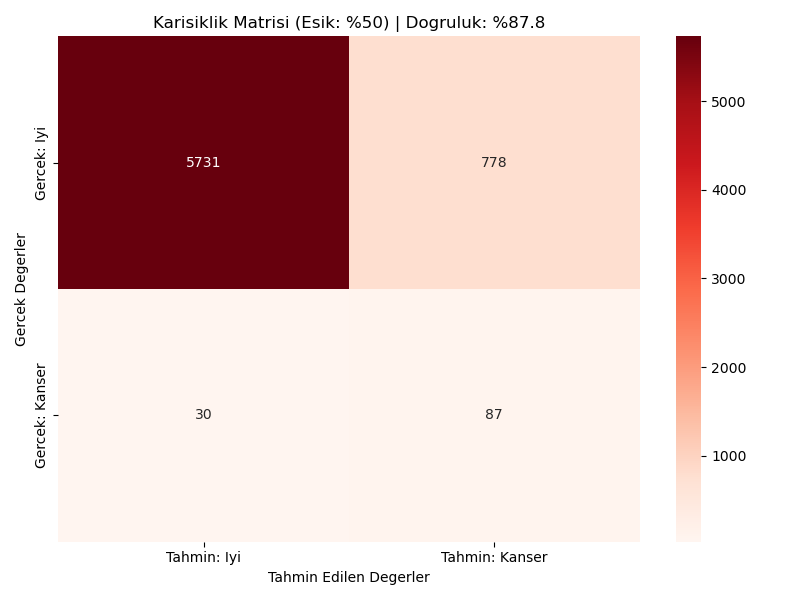
\includegraphics[width=\textwidth]{confusion_matrix_50.png}
        \caption{\%50 Karar Sınırı}
        \label{fig:cm50}
    \end{subfigure}
    \hfill
    \begin{subfigure}[b]{0.32\textwidth}
        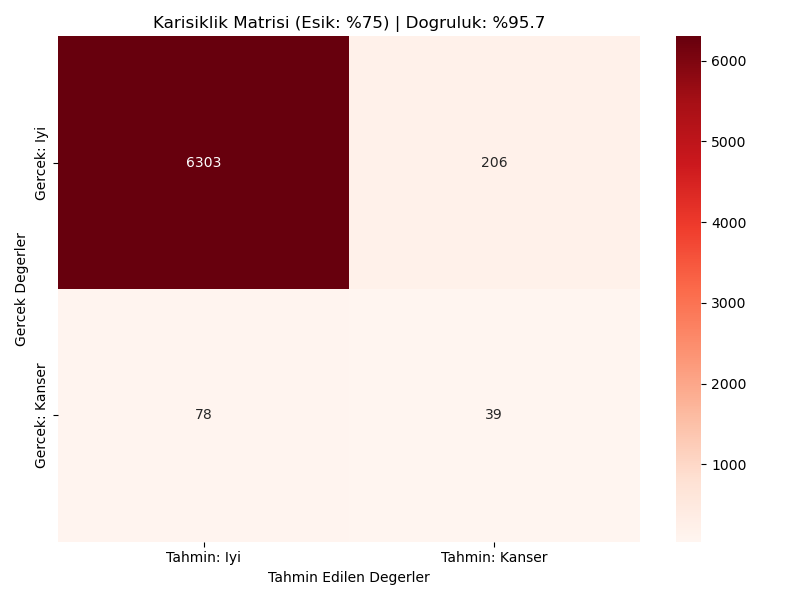
\includegraphics[width=\textwidth]{confusion_matrix_75.png}
        \caption{\%75 Karar Sınırı}
        \label{fig:cm75}
    \end{subfigure}
    \hfill
    \begin{subfigure}[b]{0.32\textwidth}
        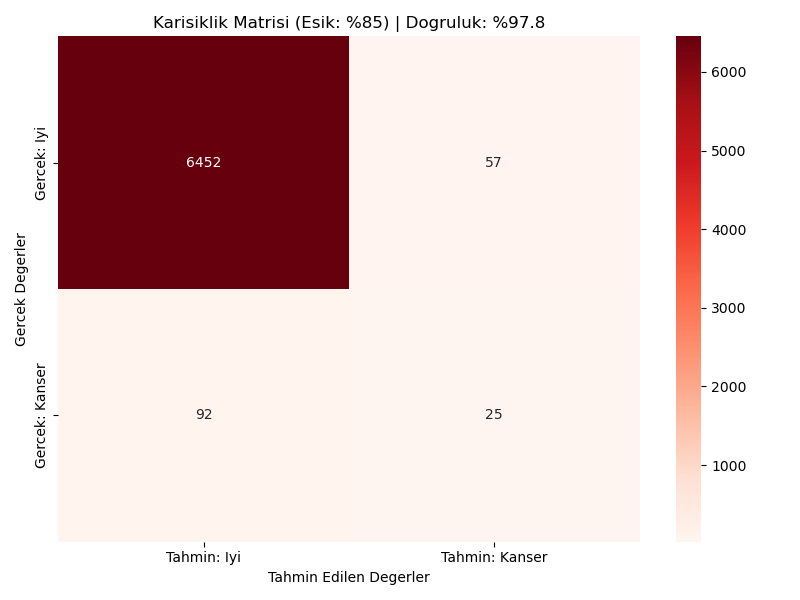
\includegraphics[width=\textwidth]{confusion_matrix_85.png}
        \caption{\%85 Karar Sınırı}
        \label{fig:cm85}
    \end{subfigure}
    \caption{Farklı Güvenlik Eşiklerinde EfficientNet-V2-S Modelinin Karmaşıklık Matrisleri}
    \label{fig:confusion_matrices}
\end{figure}

\subsection{ROC Eğrisi Analizi}
Modelin melanomu iyi huylu lezyonlardan ayırt etme gücünü gösteren ROC eğrisi ve Eğri Altı Alanı (AUC) Şekil~\ref{fig:roc_curve} üzerinde sunulmuştur.

\begin{figure}[H]
    \centering
    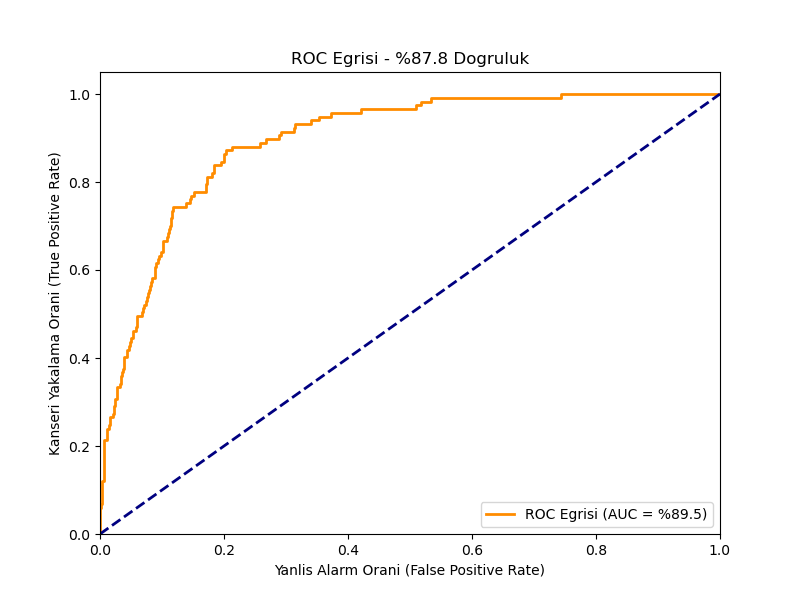
\includegraphics[width=0.6\textwidth]{roc_curve.png}
    \caption{Doğrulama Kümesi Üzerinde EfficientNet-V2-S Modelinin ROC-AUC Eğrisi}
    \label{fig:roc_curve}
\end{figure}

\subsection{Eğitim Dinamikleri ve Ezberleme Analizi}
Eğitim süresince modellerin kayıp (loss) ve doğruluk değişimleri incelenmiştir. Şekil~\ref{fig:model_karsilastirma}'de görüldüğü üzere, modeller 10. epoch'tan itibaren eğitim kaybını düşürmeye devam ederken doğrulama kayıpları yükselişe geçmiştir. Bu durum, veri seti boyutunun ve çeşitliliğinin kısıtlı olması nedeniyle modellerin ezberlemeye (overfitting) eğilim gösterdiğini ortaya koymuştur. EfficientNet-V2-S modeli en yüksek performansına henüz 1. epoch sonunda ulaşmış ve sonraki dönemlerde doğrulama başarısı gerilemiştir. ResNet-50 ise en yüksek başarısına 5. epoch sonunda ulaşmış ve 8. epoch'tan itibaren ezberlemeye başlamıştır.

\begin{figure}[H]
    \centering
    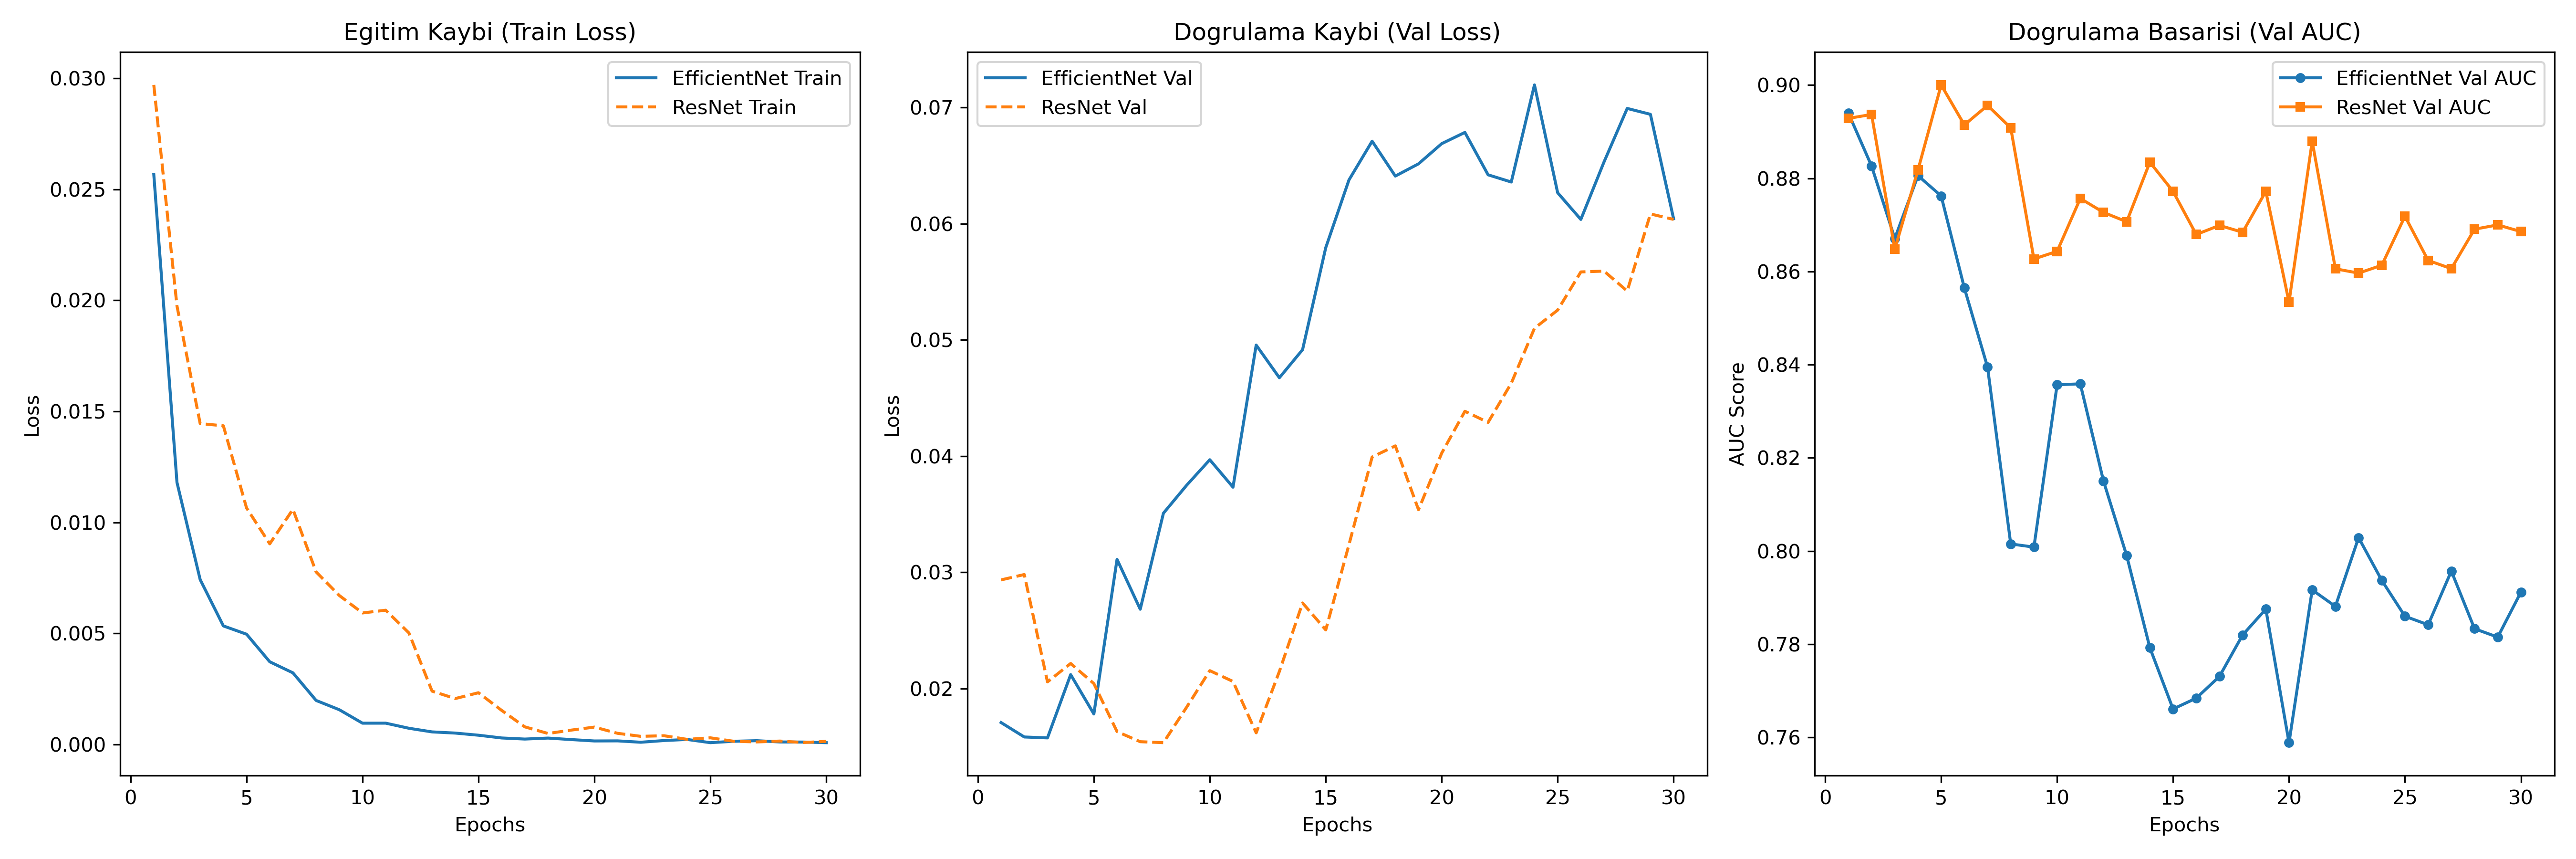
\includegraphics[width=1.0\textwidth]{model_karsilastirma.png}
    \caption{EfficientNet-V2-S ve ResNet-50 Modellerinin 30 Epochluk Eğitim Dinamikleri Karşılaştırması}
    \label{fig:model_karsilastirma}
\end{figure}

\section{Tartışma}
\label{sec:tartisma}

\subsection{Temel Bulgular}
Çalışmada elde edilen en önemli bulgu, tıbbi görüntü sınıflandırma görevlerinde genel doğruluğun (Accuracy) yanıltıcı olabileceğidir. Örneğin Tablo~\ref{tab:esik_analizi}'de görüldüğü gibi, \%85 eşik değeri modeli oldukça çekingen yapmakta ve genel doğruluğu \%97,75 gibi mükemmel görünen bir seviyeye çıkarmaktadır. Ancak bu durumda model, mevcut kanser vakalarının \%78,6'sını (117 kanser vakasından 92'sini) sağlıklı olarak etiketlemekte ve hayati bir risk yaratmaktadır (FN=92).

\subsection{Önceki Çalışmalarla Karşılaştırma}
Esteva~\cite{esteva2017} ve Brinker~\cite{brinker2019} gibi öncü tıbbi yapay zeka çalışmalarında da vurgulandığı üzere, klinik tarama aşamasında asıl amaç kanserli bir hastayı kesinlikle kaçırmamaktır. Sağlıklı bir insana şüpheli olarak yanlış alarm (False Positive) verilmesi kabul edilebilir ve tolere edilebilir bir maliyet iken, kanserli hastaya sağlıklı denilmesi doğrudan yaşam kaybına neden olabilir. Bu nedenle tarama amacıyla kullanılacak bir CAD sisteminin kesinlikle \%50 veya daha düşük karar sınırında (Recall = \%74,36, FN = 30) çalıştırılması klinik etiğin bir gereğidir.

\subsection{Klinik Çıkarımlar}
Önerilen EfficientNet-V2-S modeli, 21 milyon parametrelik kompakt yapısı sayesinde yüksek bellek gerektirmeden klinikteki lokal bilgisayarlarda veya entegre dermoskopi cihazlarında rahatlıkla çalıştırılabilir. Apple Silicon (MPS) ve CUDA desteğiyle saniyeler içinde karar vererek dermatologlara objektif bir ikinci görüş (second opinion) sunabilir.

\subsection{Sınırlılıklar}
Çalışmanın en büyük kısıtı, modellerin 10. epoch'tan sonra belirgin şekilde ezberlemeye başlamasıdır. Ayrıca ISIC 2020 veri seti tek bir yarışma formatında sunulmakta olup, farklı popülasyonlardan alınacak bağımsız veri kümeleriyle harici doğrulama (external validation) yapılması klinik kabul için şarttır.

\subsection{Gelecek Çalışmalar}
Gelecek hedeflerimiz arasında:
\begin{itemize}
    \item Modelin kararlarını klinisyen için açıklanabilir kılmak adına Grad-CAM tabanlı dikkat haritaları (attention maps) eklemek,
    \item Hastanın yaş, cinsiyet ve anatomik lezyon konumu gibi meta verilerini (metadata) görüntü öznitelikleriyle birleştiren çok modlu (multimodal) yapılar kurmak yer almaktadır.
\end{itemize}

\section{Sonuç}
\label{sec:sonuc}

Bu çalışmada, dermoskopik görüntüler üzerinden melanom teşhisi için EfficientNet-V2-S ve ResNet-50 mimarilerini kullanan transfer öğrenme tabanlı yüksek performanslı bir ikili sınıflandırma sistemi başarıyla geliştirilmiştir. Sınıf dengesizliği engelini aşmak amacıyla Focal Loss ve Ağırlıklı Rastgele Örnekleme yöntemleri entegre edilmiştir. Deneysel sonuçlar, \%89,40 AUC-ROC skoru ve \%74,36 hassasiyet oranıyla, önerilen sistemin dermatologlara teşhis aşamasında objektif bir asistan olarak destek sunabileceğini ve klinik güvenliği artırabileceğini ortaya koymuştur.

\section*{Teşekkür}
Bu araştırma ve geliştirme süreci boyunca sağladığı değerli rehberliği, akademik denetimleri ve kıymetli katkıları nedeniyle Sayın Dr. Öğr. Üyesi Nihan Özbaltan hocasına içten şükranlarımızı sunarız.

\newpage

\begin{thebibliography}{99}

\bibitem{esteva2017}
Esteva, A., Kuprel, B., Novoa, R. A., Ko, J., Swetter, S. M., Blau, H. M., \& Thrun, S. (2017). Dermatologist-level classification of skin cancer with deep neural networks. \textit{Nature}, 542(7639), 115--118. \url{https://doi.org/10.1038/nature21056}

\bibitem{haenssle2018}
Haenssle, H. A., Fink, C., Schneiderbauer, R., Toberer, F., Buhl, T., Blum, A., Kalloo, A., Hassen, A. B. H., Thomas, L., Enk, A., \& Uhlmann, L. (2018). Man against machine: diagnostic performance of a deep learning convolutional neural network for dermoscopic melanoma recognition in comparison to 58 dermatologists. \textit{Annals of Oncology}, 29(8), 1836--1842. \url{https://doi.org/10.1093/annonc/mdy166}

\bibitem{brinker2019}
Brinker, T. J., Hekler, A., Enk, A. H., Berking, C., Haferkamp, S., Hauschild, A., Weichenthal, M., Klode, J., Schadendorf, D., Holland-Letz, T., von Kalle, C., Fröhling, S., Schilling, B., \& Utikal, J. S. (2019). Deep neural networks are superior to dermatologists in melanoma image classification. \textit{European Journal of Cancer}, 119, 11--17. \url{https://doi.org/10.1016/j.ejca.2019.05.023}

\bibitem{tan2019}
Tan, M., \& Le, Q. V. (2019). EfficientNet: Rethinking model scaling for convolutional neural networks. In \textit{Proceedings of the 36th International Conference on Machine Learning (ICML)}, 97, 6105--6114. PMLR. \url{http://proceedings.mlr.press/v97/tan19a.html}

\bibitem{tan2021}
Tan, M., \& Le, Q. V. (2021). EfficientNetV2: Smaller models and faster training. In \textit{Proceedings of the 38th International Conference on Machine Learning (ICML)}, 139, 10096--10106. PMLR. \url{https://proceedings.mlr.press/v139/tan21a.html}

\bibitem{lin2017}
Lin, T. Y., Goyal, P., Girshick, R., He, K., \& Dollár, P. (2017). Focal loss for dense object detection. In \textit{Proceedings of the IEEE International Conference on Computer Vision (ICCV)}, 2980--2988. \url{https://doi.org/10.1109/ICCV.2017.324}

\bibitem{rotemberg2021}
Rotemberg, V., Kurtansky, N., Betz-Stablein, B., Caffery, L., Chousakos, E., Codella, N., Combalia, M., Dusza, S., Guitera, P., Gutman, D., Halpern, A., Helba, B., Kittler, H., Kose, K., Langer, S., Lioprys, K., Malvehy, J., Musthaq, S., Nanda, J., Nova, R., Oxholm, P., Sarantopoulos, G., Shih, G., Torresani, L., Vemula, P., Weber, S., West, D. P., Soyer, H. P., Marchetti, M. A., \& Codella, N. C. F. (2021). A patient-centric dataset of images and metadata for identifying melanomas using clinical context. \textit{Scientific Data}, 8(1), 34. \url{https://doi.org/10.1038/s41597-021-00815-z}

\bibitem{tschandl2018}
Tschandl, P., Rosendahl, C., \& Kittler, H. (2018). The HAM10000 dataset, a large collection of multi-source dermatoscopic images of common pigmented skin lesions. \textit{Scientific Data}, 5(1), 180161. \url{https://doi.org/10.1038/sdata.2018.161}

\bibitem{he2016}
He, K., Zhang, X., Ren, S., \& Sun, J. (2016). Deep residual learning for image recognition. In \textit{Proceedings of the IEEE Conference on Computer Vision and Pattern Recognition (CVPR)}, 770--778. \url{https://doi.org/10.1109/CVPR.2016.90}

\bibitem{kaggle2020}
Deotte, C. (2020). JPEG melanoma 256$\times$256. Kaggle Dataset. \url{https://www.kaggle.com/datasets/cdeotte/jpeg-melanoma-256x256}

\end{thebibliography}

\end{document}
